\documentclass[a4paper]{report}
\usepackage[utf8]{inputenc}
\usepackage[portuguese]{babel}
\usepackage{hyperref}
\usepackage{a4wide}
\hypersetup{pdftitle={SRCR - Trabalho Individual},
pdfauthor={José Ferreira},
colorlinks=true,
urlcolor=blue,
linkcolor=black}
\usepackage{subcaption}
\usepackage[cache=false]{minted}
\usepackage{listings}
\usepackage{booktabs}
\usepackage{multirow}
\usepackage{appendix}
\usepackage{tikz}
\usepackage{authblk}
\usepackage{bashful}
\usepackage{verbatim}
\usepackage{amsmath}
\usepackage{tikz}
\usepackage{tikz,fullpage}
\usepackage{pgfgantt}
\usepackage{amssymb}
\usepackage{multirow}
\usepackage{mwe}
\usetikzlibrary{arrows,%
                petri,%
                topaths}%
\usepackage{tkz-berge}
\usetikzlibrary{positioning,automata,decorations.markings}
\AfterEndEnvironment{figure}{\noindent\ignorespaces}
\AfterEndEnvironment{table}{\noindent\ignorespaces}

\definecolor{solarized@base03}{HTML}{002B36}
\definecolor{solarized@base02}{HTML}{073642}
\definecolor{solarized@base01}{HTML}{586e75}
\definecolor{solarized@base00}{HTML}{657b83}
\definecolor{solarized@base0}{HTML}{839496}
\definecolor{solarized@base1}{HTML}{93a1a1}
\definecolor{solarized@base2}{HTML}{EEE8D5}
\definecolor{solarized@base3}{HTML}{FDF6E3}
\definecolor{solarized@yellow}{HTML}{B58900}
\definecolor{solarized@orange}{HTML}{CB4B16}
\definecolor{solarized@red}{HTML}{DC322F}
\definecolor{solarized@magenta}{HTML}{D33682}
\definecolor{solarized@violet}{HTML}{6C71C4}
\definecolor{solarized@blue}{HTML}{268BD2}
\definecolor{solarized@cyan}{HTML}{2AA198}
\definecolor{solarized@green}{HTML}{859900}

\lstset{
  language=Java,
  upquote=true,
  columns=fixed,
  tabsize=4,
  extendedchars=true,
  breaklines=true,
  numbers=left,
  numbersep=5pt,
  rulesepcolor=\color{solarized@base03},
  numberstyle=\tiny\color{solarized@base01},
  basicstyle=\footnotesize\ttfamily,
  keywordstyle=\color{solarized@green},
  stringstyle=\color{solarized@yellow}\ttfamily,
  identifierstyle=\color{solarized@blue},
  commentstyle=\color{solarized@base01},
  emphstyle=\color{solarized@red}
}

\begin{document}

\title{Sistemas de Representação de Conhecimento e Raciocínio\\
\large Trabalho Individual}
\author{José Ferreira (A83683)}
\date{\today}

\begin{center}
    \begin{minipage}{0.75\linewidth}
        \centering
        
\includegraphics[width=0.4\textwidth]{images/eng.jpeg}\par\vspace{1cm}
        \vspace{1.5cm}
        \href{https://www.uminho.pt/PT}
        {\color{black}{\scshape\LARGE Universidade do Minho}} \par
        \vspace{1cm}
        \href{https://www.di.uminho.pt/}
        {\color{black}{\scshape\Large Departamento de Informática}} \par
        \vspace{1.5cm}
        \maketitle
    \end{minipage}
\end{center}

\tableofcontents

\chapter{Introdução}
Este projeto prático individual foi desenvolvido no âmbito da cadeira de
Sistemas de Representação de Conhecimento e Raciocínio.\\
O objetivo deste trabalho é aplicar os conhecimentos lecionados ao longo deste
semestre num caso de estudo.\\
Assim, será utilizada a linguagem de programação lógica \textit{Prolog} para
criar um conjunto predicados que respondem a questões relativas a dados sobre o
sistema de transportes do concelho de Oeiras.\\
Devido à natureza dos dados apresentados, a maneira como estes são melhor
representados é através de um grafo em que os nodos são as paragens e as arestas
são as ligações entre elas.\\
Ao longo deste relatório será descrito o processo utilizado para resolver o
problema.\\

\chapter{Base de Conhecimento}
Todos os dados necessários relativos às paragens de autocarros estão
disponibilizados em dois ficheiros \textit{.xlsx}.\\
O primeiro ficheiro contém informação relativa a cada uma das paragens. O
segundo ficheiro contém informação sobre a ligação entre as paragens.\\

\section{Script}
O formato de ficheiros fornecido não é suportado diretamente pelo
\textit{Prolog} por isso foi criado um \textit{script} em \textit{Python}
(Anexo \ref{app:script}) para converter os ficheiros de dados fornecidos para um
formato suportado.\\
Para conseguir ler os ficheiros \textit{.xlsx} foi utilizada a biblioteca
\textit{pandas}. Esta escolha foi feita devido à grande diversidade de formatos
suportados e fácil desenvolvimento do programa pretendido.\\
Para obter um guia de utilização do programa basta correr:\\
\textit{python
parser.py}.

\subsection{Nodos}
Para ler a informação relativa às paragens de autocarros é carregado o ficheiro
\textit{paragens\_autocarros\_oeiras\_processado\_4.xslx}. Em seguida, a tabela
é percorrida linha a linha. Para cada linha, obtém-se os seguintes dados:

\begin{itemize}
            \item gid,
            \item latitude
            \item longitude
            \item Estado de Conservacao
            \item Tipo de Abrigo
            \item Abrigo com Publicidade?
            \item Operadora
            \item Carreira
            \item Codigo de Rua
            \item Nome da Rua
            \item Freguesia
\end{itemize}
Visto que o \textit{Prolog} não suporta \textit{UTF-8} e que o próprio ficheiro
\textit{.xslx} tinha alguns problemas de \textit{encoding}, foi necessário
tratar alguns dos dados obtidos.\\
Para aqueles que apresentavam problemas de \textit{encoding} no próprio ficheiro de
dados, foi utilizada uma biblioteca de \textit{Python} chamada \textit{ftfy}
capaz de corrigir estes erros.\\
Para resolver o problema de \textit{Prolog} não suportar \textit{UTF-8} foi
utilizada uma biblioteca chamada \textit{unidecode} que contém um método para
converter uma string de \textit{UTF-8} para \textit{ASCII} convertendo os
caracteres com acentos para caracteres sem acentos.\\
Depois desta correção ser aplicada, foi detetado que algumas listas de Carreiras
tinham mais do que uma vírgula seguida. Para corrigir este problema, separamos a
string pelo carácter \textit{','}, eliminamos todas as strings vazias da lista e
voltamos a juntar todas as strings numa só com \textit{','}.\\
Estes dados recolhidos e tratados são então impressos para \textit{stdout}
seguindo o seguinte formato:\\
\textit{paragem(gid,latitude,longitude,Estado de Conservacao,Tipo de
Abrigo,Abrigo com Publicidade?,Operadora,[Carreira],Codigo de Rua,Nome da
Rua,Freguesia).}\\
Note se que já segue o formato de uma base de conhecimento em \textit{Prolog}.
Assim, basta redirecionar o \textit{output} para um ficheiro e carregar esse
ficheiro diretamente.\\

\subsection{Arestas}
O ficheiro de \textit{.xslx} fornecido com informação sobre a ligação entre cada
paragem segue o formato de ter uma \textit{Sheet} para cada percurso de
autocarro.\\
Assim, é necessário primeiro carregar o ficheiro
\textit{lista\_adjacencias\_paragens.xslx}. Depois, percorrer cada
\textit{Sheet}, e para cada \textit{Sheet} percorrer cada linha.\\
Em cada linha obtém-se o \textit{gid} atual, a carreira a que corresponde e as
coordenadas da paragem. Obtém-se também o \textit{gid} e as coordenadas da
paragem na linha seguinte. Com estes dados é possível calcular qual é a
distância entre as duas paragens.\\
O resto da informação contida neste ficheiro pode ser ignorada porque está
repetida do ficheiro relativo às paragens e já foi carregada para a base de
conhecimento.\\
Da mesma forma como foi feito para o caso das paragens, esta parte do
\textit{script} imprime \textit{Prolog} válido para o \textit{stdout} que
segue o formato:\\
\textit{edge(gid\_row, gid\_next\_row, carreira, distancia).}\\
Assim é possível obter todas as arestas do grafo que representa o problema.\\

\chapter{Predicados}
Os predicados desenvolvidos devem ser capazes de cumprir os seguintes
requisitos:

\begin{enumerate}
    \item Calcular um trajeto entre dois pontos;
    \item Selecionar apenas uma lista de operadores para um dado percurso;
    \item Excluir uma lista de operadores para o percurso;
    \item Identificar as paragens com mais carreiras num determinado percurso.
    \item Escolher o percurso com menor número de paragens;
    \item Escolher o percurso mais curto;
    \item Escolher o percurso que passe apenas por abrigos com publicidade;
    \item Escolher o percurso que passe apenas por paragens abrigadas;
    \item Escolher um ou mais pontos intermédios por onde o percurso deverá passar.
\end{enumerate}
Ao longo deste capítulo será descrita a forma como estes predicados foram
implementados.

\section{Calcular um trajeto entre dois pontos}
\subsection{Pesquisa não Informada - Depth-First}
O predicado \textit{dfs/3} implementa \textit{Depth-First search} com uma lista de
nodos visitados.\\
O predicado \textit{dfsr/4} funciona como um predicado auxiliar recursivo para
calcular o caminho. Quando este é chamado pela primeira vez é chamado com os
parâmetros: nodo de origem, nodo de destino, uma lista de visitados com o nodo
de origem e o caminho.\\
Sempre que este predicado é visitado, obtém-se o próximo nodo garantindo-se que
este é adjacente com o predicado \textit{adjacente/2}, garante-se que o nodo ainda não foi
visitado como predicado member e por fim aplica-se recursivamente o predicado
atualizando os valores.
\begin{lstlisting}[language=Prolog]
dfs(Nodo, Destino, [Nodo|Caminho]):-
    dfsr(Nodo, Destino, [Nodo], Caminho).

dfsr(Nodo, Destino, Visited, [Destino]):-
    adjacente(Nodo, Destino).

dfsr(Nodo, Destino, Visited, [ProxNodo|Caminho]):-
    adjacente(Nodo, ProxNodo),
    \+ member(ProxNodo, Visited),
    dfsr(ProxNodo, Destino, [Nodo|Visited], Caminho).

adjacente(Nodo,ProxNodo):-
    edge(Nodo, ProxNodo, _, _).
\end{lstlisting}

\begin{figure}[H]
    \centering 
    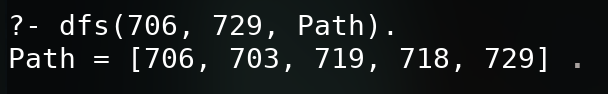
\includegraphics[width=0.4\textwidth]{images/dfs.png}
    \caption{Exemplo de Depth-First}
\end{figure}

\subsection{Pesquisa Informada - Greedy}
O predicado \textit{greedy} implementa a pesquisa gulosa. Nesta pesquisa foi
utilizado como predicado para calcular o custo estimado para chegar ao destino a
distância euclidiana.\\

\begin{lstlisting}[language=Prolog]
greedy(Nodo, Destino, Caminho/Custo):-
    estima(Nodo, Destino, E),
    agreedy([[Nodo]/0/E], InvCaminho/Custo/_, Destino),
    inverso(InvCaminho,Caminho).

agreedy(Caminhos, Caminho, Destino):-
    get_best_g(Caminhos,Caminho),
    Caminho = [Nodo|_]/_/_,
    Nodo == Destino.

agreedy(Caminhos, SolucaoCaminho, Destino):-
    get_best_g(Caminhos, MelhorCaminho),
    seleciona(MelhorCaminho,Caminhos,OutrosCaminhos),
    expand_greedy(MelhorCaminho,ExpCaminhos, Destino),
    append(OutrosCaminhos,ExpCaminhos,NovoCaminhos),
    agreedy(NovoCaminhos,SolucaoCaminho, Destino).

get_best_g([Caminho],Caminho):- !.

get_best_g([Caminho1/Custo1/Est1,_/Custo2/Est2|Caminhos], MelhorCaminho):-
    Est1 =< Est2,
    !,
    get_best_g([Caminho1/Custo1/Est1|Caminhos],MelhorCaminho).

get_best_g([_|Caminhos], MelhorCaminho):-
    get_best_g(Caminhos, MelhorCaminho).

expand_greedy(Caminho, ExpCaminhos, Destino):-
    findall(NovoCaminho, adjacente(Caminho, NovoCaminho, Destino), ExpCaminhos).

estima(P1,P2,R):-
        paragem(P1,X1,Y1,_,_,_,_,_,_,_,_),
        paragem(P2,X2,Y2,_,_,_,_,_,_,_,_),
        R is sqrt(((X1-X2)*(X1-X2))+((Y1-Y2)*(Y1-Y2))).

adjacente([Nodo|Caminho]/Custo/_, [ProxNodo,Nodo|Caminho]/NovoCusto/Est, Destino):-
    edge(Nodo, ProxNodo, _, PassoCusto),
    \+ member(ProxNodo, Caminho),
    NovoCusto is Custo + PassoCusto,
    estima(ProxNodo, Destino, Est).
\end{lstlisting}

\begin{figure}[H]
    \centering 
    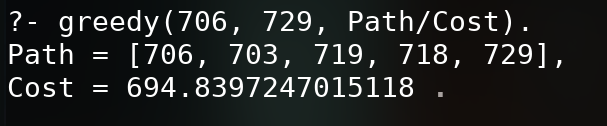
\includegraphics[width=0.4\textwidth]{images/greedy.png}
    \caption{Exemplo de Greedy}
\end{figure}

\subsection{Depth-First vs Greedy}
Ambas os métodos de pesquisa implementados não garantem a completude da solução.
No caso de \textit{Depth-First} falha em espaços de profundidade infinita com
\textit{loops}, no caso da \textit{Greedy} pode entrar em ciclos e é susceptível
a falsos começos.\\
Apesar de a complexidade temporal parecer a mesma à primeira vista (O($b^m$)), p
tempo do algoritmo \textit{Greedy} pode ser consideravelmente diminuído com uma
boa função heurística. No melhor caso porde chegar a (O(bd)).\\
No caso da complexidade no espaço a melhor é a \textit{Depth-First} fazendo com
que esta tenha espaço linear.\\
Por fim, no caso da Optimalidade da solução encontrada, nenhum destes algoritmos
a garante. O \textit{Depth-First} devolve a primeira solução encontrada e o
\textit{Greedy} pode não encontrar a solução óptima.

\begin{table}[H]
\begin{tabular}{|l|l|l|l|l|l|}
\hline
            & Completude & Complexidade no Tempo   & Complexidade no Espaço  & Optimalidade \\ \hline
Depth-First & Não        & O($b^m$)                & O(bm)                   & Não          \\ \hline
    Greedy      & Não        & O($b^m$) / O(bd)    & O($b^m$)                & Não          \\ \hline
\end{tabular}
\end{table}

\section{Selecionar apenas uma lista de operadores para um dado percurso}
Para obter um percurso que só utiliza um determinado conjunto de operadores
basta modificar o método de pesquisa \textit{Depth-First} para garantir que o operador está na
lista.\\
Desta forma, foi desenvolvido o predicado \textit{dfs\_op/4}

\begin{lstlisting}[language=Prolog]
dfs_op(Nodo, Destino, Operadoras, [Nodo|Caminho]):-
    dfsr_op(Nodo, Destino, Operadoras, [Nodo], Caminho).

dfsr_op(Nodo, Destino, Operadoras, Visited, [Destino]):-
    adjacente(Nodo, Destino),
    paragem(Nodo,_,_,_,_,_,O,_,_,_,_),
    member(O,Operadoras).

dfsr_op(Nodo, Destino, Operadoras, Visited, [ProxNodo|Caminho]):-
    adjacente(Nodo, ProxNodo),
    \+ member(ProxNodo, Visited),
    paragem(Nodo,_,_,_,_,_,O,_,_,_,_),
    member(O,Operadoras),
    dfsr_op(ProxNodo, Destino, Operadoras, [Nodo|Visited], Caminho).
\end{lstlisting}

\begin{figure}[H]
    \centering 
    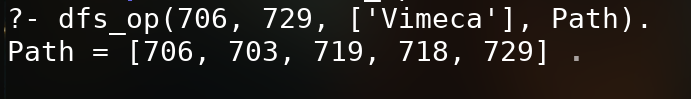
\includegraphics[width=0.5\textwidth]{images/dfs_op.png}
    \caption{Exemplo de dfs\_op}
\end{figure}

\section{Excluir uma lista de operadores para o percurso}
De forma análoga, para garantir que o percurso não utiliza um determinado
conjunto de operadores, basta modificar o método de pesquisa
\textit{Depth-First} para garantir que o operador não está na lista. Para tal
basta negar a linha criada para o predicado descrito acima.\\

\begin{lstlisting}[language=Prolog]
dfs_noop(Nodo, Destino, Operadoras, [Nodo|Caminho]):-
    dfsr_op(Nodo, Destino, Operadoras, [Nodo], Caminho).

dfsr_noop(Nodo, Destino, Operadoras, Visited, [Destino]):-
    adjacente(Nodo, Destino).

dfsr_noop(Nodo, Destino, Operadoras, Visited, [ProxNodo|Caminho]):-
    adjacente(Nodo, ProxNodo),
    \+ member(ProxNodo, Visited),
    paragem(Nodo,_,_,_,_,_,O,_,_,_,_),
    \+ member(O,Operadoras),
    dfsr_noop(ProxNodo, Destino, Operadoras, [Nodo|Visited], Caminho).
\end{lstlisting}

\begin{figure}[H]
    \centering 
    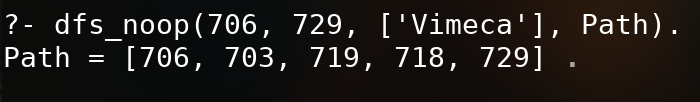
\includegraphics[width=0.5\textwidth]{images/dfs_noop.png}
    \caption{Exemplo de dfs\_noop}
\end{figure}

\section{Identificar as paragens com mais carreiras num determinado percurso}
Para identificar as paragens com mais carreiras num determinado percurso foi
criado o predicado \textit{sorted\_nstop/3}.\\
Primeiro é calculado um percurso com base num predicado à escolha. Neste caso
foi usado o \textit{dfs/3}. Em seguida utiliza-se o predicado \textit{calc\_len}
para calcular uma lista de tuplos com o nodo e o número de Carreiras em cada
nodo.\\
Por fim foi implementado uma variação do \textit{QuickSort} que organiza em
sentido decrescente com base no segundo elemento do tuplo. A única alteração que
foi feita ao algoritmo foi na função que calcula o pivô fazendo com que o termo
de comparação seja o segundo elemento do tuplo.\\

\begin{lstlisting}[language=Prolog]
sorted_nstop(Nodo, Destino, R):-
    dfs(Nodo, Destino, P),
    calc_len(P, PL),
    quick_sort(PL, R).

calc_len([], []).
calc_len([H|T], [(H,LC)|R]):-
    paragem(H,_,_,_,_,_,_,C,_,_,_),
    length(C, LC),
    calc_len(T, R).

quick_sort([],[]).
quick_sort([H|T],Sorted):-
	pivoting(H,T,L1,L2),
        quick_sort(L1,Sorted1),
        quick_sort(L2,Sorted2),
	append(Sorted1,[H|Sorted2], Sorted).
   
pivoting(H,[], [], []).
pivoting((H,C1),[(X,C2)|T], L, [(X,C2)|G]):-
    C2=<C1,
    pivoting((H,C1),T,L,G).
pivoting((H, C1),[(X,C2)|T], [(X, C2)|L], G):-
    C2>C1,
    pivoting((H,C1), T, L, G).
\end{lstlisting}

\begin{figure}[H]
    \centering 
    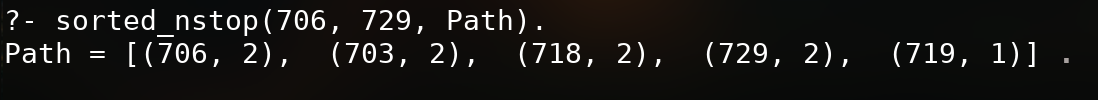
\includegraphics[width=0.6\textwidth]{images/sorted_nstop.png}
    \caption{Exemplo de sorted\_nstop}
\end{figure}

\section{Escolher o percurso com menor número de paragens}
Para calcular o caminho com o menor número de paragens foi criado o predicado
\textit{dfs\_len/4} que utiliza \textit{Depth-First} e depois calcula o
comprimento do caminho calculado. Este predicado é utilizado em conjunto com o
\textit{findall/3} para obter todos os caminhos possíveis da origem até ao
destino.\\
Em seguida é utilizado o predicado \textit{minimo/2} para obter o mínimo.\\
Isto é conjugado para criar o predicado \textit{best\_len/4}.

\begin{lstlisting}[language=Prolog]
best_len(Nodo, Destino, S, N_stops) :-
    findall((SS, CC), dfs_len(Nodo, Destino, SS, CC), L),
    minimo(L,(S,N_stops)).

dfs_len(Nodo, Destino, C, N):-
    dfs(Nodo, Destino, C),
    length(C, N).

minimo([H|T], R):- minimoa(T, H, R).

minimoa([], Min, Min).
minimoa([(_, C) | T], (NM, CM), Min):-
    C > CM,
    minimoa(T, (NM, CM) , Min).

minimoa([(H, C) | T], (_, CM), Min):-
    C =< CM,
    minimoa(T, (H, C), Min).
\end{lstlisting}
Infelizmente este método entra em \textit{loop} infinito possivelmente devido a
informação repetida na base de conhecimento.

\section{Escolher o percurso mais curto}
De forma semelhante, o predicado \textit{beat\_cost/4} calcula o caminho com
menor custo. Sendo que a única diferença quando comparado com a
\textit{best\_len/4} é que calcula o custo do caminho em vez de calcular o
comprimento.

\begin{lstlisting}[language=Prolog]
best_cost(Nodo, Destino, S, Custo):-
    findall((SS, CC), dfs_cost(Nodo, Destino, SS, CC), L),
    minimo(L,(S,Custo)).

dfs_cost(Nodo, Destino, Path, Custo):-
    dfs(Nodo, Destino, Path),
    calc_cost(Path, Custo).

calc_cost([H,NH], C):-
    edge(H, NH, _, C).
calc_cost([H,NH|T], C):-
    edge(H, NH, _, C1),
    calc_cost([NH|T], C2),
    C is C1+ C2.
\end{lstlisting}
Infelizmente este método entra em \textit{loop} infinito possivelmente devido a
informação repetida na base de conhecimento.

\section{Escolher o percurso que passe apenas por abrigos com publicidade}
Como foi feito acima, para garantir que o percurso não utiliza abrigos sem
publicidade, basta modificar o método de pesquisa \textit{Depth-First} para
garantir que a característica da paragem. Assim foi desenvolvido o predicado
\textit{dfs\_pub/3}.\\

\begin{lstlisting}[language=Prolog]
dfs_pub(Nodo, Destino, [Nodo|Caminho]):-
    dfsr_abrigado(Nodo, Destino, [Nodo], Caminho).

dfsr_pub(Nodo, Destino, _, [Destino]):-
    adjacente(Nodo, Destino).

dfsr_pub(Nodo, Destino, Visited, [ProxNodo|Caminho]):-
    adjacente(Nodo, ProxNodo),
    \+ member(ProxNodo, Visited),
    paragem(Nodo,_,_,_,_,_,_,P,_,_,_),
    P == 'Yes',
    dfsr_pub(ProxNodo, Destino, [Nodo|Visited], Caminho).
\end{lstlisting}

\begin{figure}[H]
    \centering 
    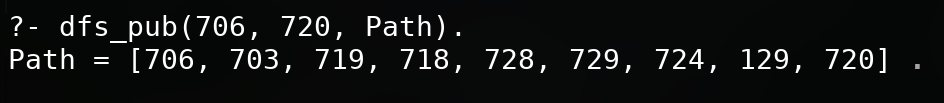
\includegraphics[width=0.5\textwidth]{images/dfs_pub.png}
    \caption{Exemplo de dfs\_pub}
\end{figure}

\section{Escolher o percurso que passe apenas por paragens abrigadas}
De forma análoga, para garantir que as paragens por onde passa o caminho sejam
todas abrigadas, basta garantir que todos os nodos têm a propriedade a ser
diferente de 'Sem Abrigo'. Desta forma, foi criado o predicado
\textit{dfs\_abrigado}.\\

\begin{lstlisting}[language=Prolog]
dfs_abrigado(Nodo, Destino, [Nodo|Caminho]):-
    dfsr_abrigado(Nodo, Destino, [Nodo], Caminho).

dfsr_abrigado(Nodo, Destino, _, [Destino]):-
    adjacente(Nodo, Destino).

dfsr_abrigado(Nodo, Destino, Visited, [ProxNodo|Caminho]):-
    adjacente(Nodo, ProxNodo),
    \+ member(ProxNodo, Visited),
    paragem(Nodo,_,_,_,_,_,A,_,_,_,_),
    A \== 'Sem Abrigo',
    dfsr_abrigado(ProxNodo, Destino, [Nodo|Visited], Caminho).
\end{lstlisting}

\begin{figure}[H]
    \centering 
    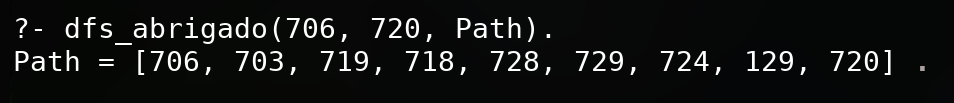
\includegraphics[width=0.5\textwidth]{images/dfs_abrigado.png}
    \caption{Exemplo de dfs\_abrigado}
\end{figure}

\section{Escolher um ou mais pontos intermédios por onde o percurso deverá passar}
A maneira como foi criado o método para calcular o caminho entre dois pontos
permite facilmente alterar o método de pesquisa utilizado. Neste caso o método
de pesquisa utilizado foi o \textit{Greedy}.\\
O predicado implementado calcula o caminho entre as duas primeiras paragens da
lista, aplica o predicado \textit{init/2} que calcula a lista menos o último
elemento, calcula recursivamente o caminho para os outros pontos e concatena as
duas listas calculadas.

\begin{lstlisting}[language=Prolog]
inter([P1, P2], Curr):-
    greedy(P1, P2, Curr/_).

inter([P1, P2 | Rest], Path):-
    greedy(P1, P2, Curr/_),
    inter([P2 | Rest], Tail),
    init(Curr, Initial),
    append(Initial, Tail, Path).

init([], []).
init([A], []).
init([H|T], [H|R]):- init(T, R).
\end{lstlisting}
Para modificar este predicado para utilizar o método de pesquisa
\textit{Depth-First} implementado bastaria alterar as linhas com o predicado
\textit{greedy/3} para:

\begin{lstlisting}[language=Prolog]
dfs(P1, P2, Curr),
\end{lstlisting}

\begin{figure}[H]
    \centering 
    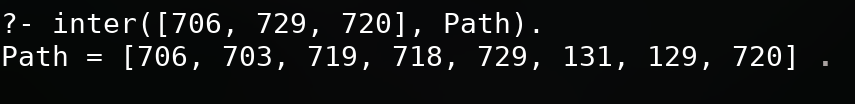
\includegraphics[width=0.6\textwidth]{images/inter.png}
    \caption{Exemplo de inter}
\end{figure}

\chapter{Conclusão}
Concluindo , com este trabalho foram aplicados os conhecimentos de
\textit{Prolog} lecionados ao longo deste semestre na unidade curricular de
sistemas de representação de conhecimento e raciocino. Nomeadamente
conhecimentos relativos a travessia de grafos.\\
Como trabalho futuro seria relevante implementar mais métodos de pesquisa
informada, nomeadamente o A*, de forma a melhorar a qualidade dos resultados
obtidos e resolver a escolha do melhor percurso com base no número de paragens e
com o comprimento.

\appendix
\chapter{Script em Python}\label{app:script}
\lstinputlisting[language=Python]{../src/parse.py}

\end{document}
